\documentclass[11pt]{article}

    \usepackage[breakable]{tcolorbox}
    \usepackage{parskip} % Stop auto-indenting (to mimic markdown behaviour)
    
    \usepackage{iftex}
    \ifPDFTeX
    	\usepackage[T1]{fontenc}
    	\usepackage{mathpazo}
    \else
    	\usepackage{fontspec}
    \fi

    % Basic figure setup, for now with no caption control since it's done
    % automatically by Pandoc (which extracts ![](path) syntax from Markdown).
    \usepackage{graphicx}
    % Maintain compatibility with old templates. Remove in nbconvert 6.0
    \let\Oldincludegraphics\includegraphics
    % Ensure that by default, figures have no caption (until we provide a
    % proper Figure object with a Caption API and a way to capture that
    % in the conversion process - todo).
    \usepackage{caption}
    %\DeclareCaptionFormat{nocaption}{}
    %\captionsetup{format=nocaption,aboveskip=0pt,belowskip=0pt}

    \usepackage{float}
    \floatplacement{figure}{H} % forces figures to be placed at the correct location
    \usepackage{xcolor} % Allow colors to be defined
    \usepackage{enumerate} % Needed for markdown enumerations to work
    \usepackage{geometry} % Used to adjust the document margins
    \usepackage{amsmath} % Equations
    \usepackage{amssymb} % Equations
    \usepackage{siunitx}
    \usepackage{textcomp} % defines textquotesingle
    % Hack from http://tex.stackexchange.com/a/47451/13684:
    \AtBeginDocument{%
        \def\PYZsq{\textquotesingle}% Upright quotes in Pygmentized code
    }
    \usepackage{upquote} % Upright quotes for verbatim code
    \usepackage{eurosym} % defines \euro
    \usepackage[mathletters]{ucs} % Extended unicode (utf-8) support
    \usepackage{fancyvrb} % verbatim replacement that allows latex
    \usepackage{grffile} % extends the file name processing of package graphics 
                         % to support a larger range
    \makeatletter % fix for old versions of grffile with XeLaTeX
    \@ifpackagelater{grffile}{2019/11/01}
    {
      % Do nothing on new versions
    }
    {
      \def\Gread@@xetex#1{%
        \IfFileExists{"\Gin@base".bb}%
        {\Gread@eps{\Gin@base.bb}}%
        {\Gread@@xetex@aux#1}%
      }
    }
    \makeatother
    \usepackage[Export]{adjustbox} % Used to constrain images to a maximum size
    \adjustboxset{max size={0.9\linewidth}{0.9\paperheight}}

    % The hyperref package gives us a pdf with properly built
    % internal navigation ('pdf bookmarks' for the table of contents,
    % internal cross-reference links, web links for URLs, etc.)
    \usepackage{hyperref}
    % The default LaTeX title has an obnoxious amount of whitespace. By default,
    % titling removes some of it. It also provides customization options.
    \usepackage{titling}
    \usepackage{longtable} % longtable support required by pandoc >1.10
    \usepackage{booktabs}  % table support for pandoc > 1.12.2
    \usepackage[inline]{enumitem} % IRkernel/repr support (it uses the enumerate* environment)
    \usepackage[normalem]{ulem} % ulem is needed to support strikethroughs (\sout)
                                % normalem makes italics be italics, not underlines
    \usepackage{mathrsfs}
    \usepackage[bold-style=TeX]{unicode-math}

    
    % Colors for the hyperref package
    \definecolor{urlcolor}{rgb}{0,.145,.698}
    \definecolor{linkcolor}{rgb}{.71,0.21,0.01}
    \definecolor{citecolor}{rgb}{.12,.54,.11}

    % ANSI colors
    \definecolor{ansi-black}{HTML}{3E424D}
    \definecolor{ansi-black-intense}{HTML}{282C36}
    \definecolor{ansi-red}{HTML}{E75C58}
    \definecolor{ansi-red-intense}{HTML}{B22B31}
    \definecolor{ansi-green}{HTML}{00A250}
    \definecolor{ansi-green-intense}{HTML}{007427}
    \definecolor{ansi-yellow}{HTML}{DDB62B}
    \definecolor{ansi-yellow-intense}{HTML}{B27D12}
    \definecolor{ansi-blue}{HTML}{208FFB}
    \definecolor{ansi-blue-intense}{HTML}{0065CA}
    \definecolor{ansi-magenta}{HTML}{D160C4}
    \definecolor{ansi-magenta-intense}{HTML}{A03196}
    \definecolor{ansi-cyan}{HTML}{60C6C8}
    \definecolor{ansi-cyan-intense}{HTML}{258F8F}
    \definecolor{ansi-white}{HTML}{C5C1B4}
    \definecolor{ansi-white-intense}{HTML}{A1A6B2}
    \definecolor{ansi-default-inverse-fg}{HTML}{FFFFFF}
    \definecolor{ansi-default-inverse-bg}{HTML}{000000}

    % common color for the border for error outputs.
    \definecolor{outerrorbackground}{HTML}{FFDFDF}

    % commands and environments needed by pandoc snippets
    % extracted from the output of `pandoc -s`
    \providecommand{\tightlist}{%
      \setlength{\itemsep}{0pt}\setlength{\parskip}{0pt}}
    \DefineVerbatimEnvironment{Highlighting}{Verbatim}{commandchars=\\\{\}}
    % Add ',fontsize=\small' for more characters per line
    \newenvironment{Shaded}{}{}
    \newcommand{\KeywordTok}[1]{\textcolor[rgb]{0.00,0.44,0.13}{\textbf{{#1}}}}
    \newcommand{\DataTypeTok}[1]{\textcolor[rgb]{0.56,0.13,0.00}{{#1}}}
    \newcommand{\DecValTok}[1]{\textcolor[rgb]{0.25,0.63,0.44}{{#1}}}
    \newcommand{\BaseNTok}[1]{\textcolor[rgb]{0.25,0.63,0.44}{{#1}}}
    \newcommand{\FloatTok}[1]{\textcolor[rgb]{0.25,0.63,0.44}{{#1}}}
    \newcommand{\CharTok}[1]{\textcolor[rgb]{0.25,0.44,0.63}{{#1}}}
    \newcommand{\StringTok}[1]{\textcolor[rgb]{0.25,0.44,0.63}{{#1}}}
    \newcommand{\CommentTok}[1]{\textcolor[rgb]{0.38,0.63,0.69}{\textit{{#1}}}}
    \newcommand{\OtherTok}[1]{\textcolor[rgb]{0.00,0.44,0.13}{{#1}}}
    \newcommand{\AlertTok}[1]{\textcolor[rgb]{1.00,0.00,0.00}{\textbf{{#1}}}}
    \newcommand{\FunctionTok}[1]{\textcolor[rgb]{0.02,0.16,0.49}{{#1}}}
    \newcommand{\RegionMarkerTok}[1]{{#1}}
    \newcommand{\ErrorTok}[1]{\textcolor[rgb]{1.00,0.00,0.00}{\textbf{{#1}}}}
    \newcommand{\NormalTok}[1]{{#1}}
    
    % Additional commands for more recent versions of Pandoc
    \newcommand{\ConstantTok}[1]{\textcolor[rgb]{0.53,0.00,0.00}{{#1}}}
    \newcommand{\SpecialCharTok}[1]{\textcolor[rgb]{0.25,0.44,0.63}{{#1}}}
    \newcommand{\VerbatimStringTok}[1]{\textcolor[rgb]{0.25,0.44,0.63}{{#1}}}
    \newcommand{\SpecialStringTok}[1]{\textcolor[rgb]{0.73,0.40,0.53}{{#1}}}
    \newcommand{\ImportTok}[1]{{#1}}
    \newcommand{\DocumentationTok}[1]{\textcolor[rgb]{0.73,0.13,0.13}{\textit{{#1}}}}
    \newcommand{\AnnotationTok}[1]{\textcolor[rgb]{0.38,0.63,0.69}{\textbf{\textit{{#1}}}}}
    \newcommand{\CommentVarTok}[1]{\textcolor[rgb]{0.38,0.63,0.69}{\textbf{\textit{{#1}}}}}
    \newcommand{\VariableTok}[1]{\textcolor[rgb]{0.10,0.09,0.49}{{#1}}}
    \newcommand{\ControlFlowTok}[1]{\textcolor[rgb]{0.00,0.44,0.13}{\textbf{{#1}}}}
    \newcommand{\OperatorTok}[1]{\textcolor[rgb]{0.40,0.40,0.40}{{#1}}}
    \newcommand{\BuiltInTok}[1]{{#1}}
    \newcommand{\ExtensionTok}[1]{{#1}}
    \newcommand{\PreprocessorTok}[1]{\textcolor[rgb]{0.74,0.48,0.00}{{#1}}}
    \newcommand{\AttributeTok}[1]{\textcolor[rgb]{0.49,0.56,0.16}{{#1}}}
    \newcommand{\InformationTok}[1]{\textcolor[rgb]{0.38,0.63,0.69}{\textbf{\textit{{#1}}}}}
    \newcommand{\WarningTok}[1]{\textcolor[rgb]{0.38,0.63,0.69}{\textbf{\textit{{#1}}}}}
    
    
    % Define a nice break command that doesn't care if a line doesn't already
    % exist.
    \def\br{\hspace*{\fill} \\* }
    % Math Jax compatibility definitions
    \def\gt{>}
    \def\lt{<}
    \let\Oldtex\TeX
    \let\Oldlatex\LaTeX
    \renewcommand{\TeX}{\textrm{\Oldtex}}
    \renewcommand{\LaTeX}{\textrm{\Oldlatex}}
    % Document parameters
    % Document title
    \title{\textbf{Documentation: Surrogate mechanics modelling}}
    \author{\href{mailto:mdan066@aucklanduni.ac.nz}{Max Dang Vu}} 
 
% Pygments definitions
\makeatletter
\def\PY@reset{\let\PY@it=\relax \let\PY@bf=\relax%
    \let\PY@ul=\relax \let\PY@tc=\relax%
    \let\PY@bc=\relax \let\PY@ff=\relax}
\def\PY@tok#1{\csname PY@tok@#1\endcsname}
\def\PY@toks#1+{\ifx\relax#1\empty\else%
    \PY@tok{#1}\expandafter\PY@toks\fi}
\def\PY@do#1{\PY@bc{\PY@tc{\PY@ul{%
    \PY@it{\PY@bf{\PY@ff{#1}}}}}}}
\def\PY#1#2{\PY@reset\PY@toks#1+\relax+\PY@do{#2}}

\@namedef{PY@tok@w}{\def\PY@tc##1{\textcolor[rgb]{0.73,0.73,0.73}{##1}}}
\@namedef{PY@tok@c}{\let\PY@it=\textit\def\PY@tc##1{\textcolor[rgb]{0.25,0.50,0.50}{##1}}}
\@namedef{PY@tok@cp}{\def\PY@tc##1{\textcolor[rgb]{0.74,0.48,0.00}{##1}}}
\@namedef{PY@tok@k}{\let\PY@bf=\textbf\def\PY@tc##1{\textcolor[rgb]{0.00,0.50,0.00}{##1}}}
\@namedef{PY@tok@kp}{\def\PY@tc##1{\textcolor[rgb]{0.00,0.50,0.00}{##1}}}
\@namedef{PY@tok@kt}{\def\PY@tc##1{\textcolor[rgb]{0.69,0.00,0.25}{##1}}}
\@namedef{PY@tok@o}{\def\PY@tc##1{\textcolor[rgb]{0.40,0.40,0.40}{##1}}}
\@namedef{PY@tok@ow}{\let\PY@bf=\textbf\def\PY@tc##1{\textcolor[rgb]{0.67,0.13,1.00}{##1}}}
\@namedef{PY@tok@nb}{\def\PY@tc##1{\textcolor[rgb]{0.00,0.50,0.00}{##1}}}
\@namedef{PY@tok@nf}{\def\PY@tc##1{\textcolor[rgb]{0.00,0.00,1.00}{##1}}}
\@namedef{PY@tok@nc}{\let\PY@bf=\textbf\def\PY@tc##1{\textcolor[rgb]{0.00,0.00,1.00}{##1}}}
\@namedef{PY@tok@nn}{\let\PY@bf=\textbf\def\PY@tc##1{\textcolor[rgb]{0.00,0.00,1.00}{##1}}}
\@namedef{PY@tok@ne}{\let\PY@bf=\textbf\def\PY@tc##1{\textcolor[rgb]{0.82,0.25,0.23}{##1}}}
\@namedef{PY@tok@nv}{\def\PY@tc##1{\textcolor[rgb]{0.10,0.09,0.49}{##1}}}
\@namedef{PY@tok@no}{\def\PY@tc##1{\textcolor[rgb]{0.53,0.00,0.00}{##1}}}
\@namedef{PY@tok@nl}{\def\PY@tc##1{\textcolor[rgb]{0.63,0.63,0.00}{##1}}}
\@namedef{PY@tok@ni}{\let\PY@bf=\textbf\def\PY@tc##1{\textcolor[rgb]{0.60,0.60,0.60}{##1}}}
\@namedef{PY@tok@na}{\def\PY@tc##1{\textcolor[rgb]{0.49,0.56,0.16}{##1}}}
\@namedef{PY@tok@nt}{\let\PY@bf=\textbf\def\PY@tc##1{\textcolor[rgb]{0.00,0.50,0.00}{##1}}}
\@namedef{PY@tok@nd}{\def\PY@tc##1{\textcolor[rgb]{0.67,0.13,1.00}{##1}}}
\@namedef{PY@tok@s}{\def\PY@tc##1{\textcolor[rgb]{0.73,0.13,0.13}{##1}}}
\@namedef{PY@tok@sd}{\let\PY@it=\textit\def\PY@tc##1{\textcolor[rgb]{0.73,0.13,0.13}{##1}}}
\@namedef{PY@tok@si}{\let\PY@bf=\textbf\def\PY@tc##1{\textcolor[rgb]{0.73,0.40,0.53}{##1}}}
\@namedef{PY@tok@se}{\let\PY@bf=\textbf\def\PY@tc##1{\textcolor[rgb]{0.73,0.40,0.13}{##1}}}
\@namedef{PY@tok@sr}{\def\PY@tc##1{\textcolor[rgb]{0.73,0.40,0.53}{##1}}}
\@namedef{PY@tok@ss}{\def\PY@tc##1{\textcolor[rgb]{0.10,0.09,0.49}{##1}}}
\@namedef{PY@tok@sx}{\def\PY@tc##1{\textcolor[rgb]{0.00,0.50,0.00}{##1}}}
\@namedef{PY@tok@m}{\def\PY@tc##1{\textcolor[rgb]{0.40,0.40,0.40}{##1}}}
\@namedef{PY@tok@gh}{\let\PY@bf=\textbf\def\PY@tc##1{\textcolor[rgb]{0.00,0.00,0.50}{##1}}}
\@namedef{PY@tok@gu}{\let\PY@bf=\textbf\def\PY@tc##1{\textcolor[rgb]{0.50,0.00,0.50}{##1}}}
\@namedef{PY@tok@gd}{\def\PY@tc##1{\textcolor[rgb]{0.63,0.00,0.00}{##1}}}
\@namedef{PY@tok@gi}{\def\PY@tc##1{\textcolor[rgb]{0.00,0.63,0.00}{##1}}}
\@namedef{PY@tok@gr}{\def\PY@tc##1{\textcolor[rgb]{1.00,0.00,0.00}{##1}}}
\@namedef{PY@tok@ge}{\let\PY@it=\textit}
\@namedef{PY@tok@gs}{\let\PY@bf=\textbf}
\@namedef{PY@tok@gp}{\let\PY@bf=\textbf\def\PY@tc##1{\textcolor[rgb]{0.00,0.00,0.50}{##1}}}
\@namedef{PY@tok@go}{\def\PY@tc##1{\textcolor[rgb]{0.53,0.53,0.53}{##1}}}
\@namedef{PY@tok@gt}{\def\PY@tc##1{\textcolor[rgb]{0.00,0.27,0.87}{##1}}}
\@namedef{PY@tok@err}{\def\PY@bc##1{{\setlength{\fboxsep}{\string -\fboxrule}\fcolorbox[rgb]{1.00,0.00,0.00}{1,1,1}{\strut ##1}}}}
\@namedef{PY@tok@kc}{\let\PY@bf=\textbf\def\PY@tc##1{\textcolor[rgb]{0.00,0.50,0.00}{##1}}}
\@namedef{PY@tok@kd}{\let\PY@bf=\textbf\def\PY@tc##1{\textcolor[rgb]{0.00,0.50,0.00}{##1}}}
\@namedef{PY@tok@kn}{\let\PY@bf=\textbf\def\PY@tc##1{\textcolor[rgb]{0.00,0.50,0.00}{##1}}}
\@namedef{PY@tok@kr}{\let\PY@bf=\textbf\def\PY@tc##1{\textcolor[rgb]{0.00,0.50,0.00}{##1}}}
\@namedef{PY@tok@bp}{\def\PY@tc##1{\textcolor[rgb]{0.00,0.50,0.00}{##1}}}
\@namedef{PY@tok@fm}{\def\PY@tc##1{\textcolor[rgb]{0.00,0.00,1.00}{##1}}}
\@namedef{PY@tok@vc}{\def\PY@tc##1{\textcolor[rgb]{0.10,0.09,0.49}{##1}}}
\@namedef{PY@tok@vg}{\def\PY@tc##1{\textcolor[rgb]{0.10,0.09,0.49}{##1}}}
\@namedef{PY@tok@vi}{\def\PY@tc##1{\textcolor[rgb]{0.10,0.09,0.49}{##1}}}
\@namedef{PY@tok@vm}{\def\PY@tc##1{\textcolor[rgb]{0.10,0.09,0.49}{##1}}}
\@namedef{PY@tok@sa}{\def\PY@tc##1{\textcolor[rgb]{0.73,0.13,0.13}{##1}}}
\@namedef{PY@tok@sb}{\def\PY@tc##1{\textcolor[rgb]{0.73,0.13,0.13}{##1}}}
\@namedef{PY@tok@sc}{\def\PY@tc##1{\textcolor[rgb]{0.73,0.13,0.13}{##1}}}
\@namedef{PY@tok@dl}{\def\PY@tc##1{\textcolor[rgb]{0.73,0.13,0.13}{##1}}}
\@namedef{PY@tok@s2}{\def\PY@tc##1{\textcolor[rgb]{0.73,0.13,0.13}{##1}}}
\@namedef{PY@tok@sh}{\def\PY@tc##1{\textcolor[rgb]{0.73,0.13,0.13}{##1}}}
\@namedef{PY@tok@s1}{\def\PY@tc##1{\textcolor[rgb]{0.73,0.13,0.13}{##1}}}
\@namedef{PY@tok@mb}{\def\PY@tc##1{\textcolor[rgb]{0.40,0.40,0.40}{##1}}}
\@namedef{PY@tok@mf}{\def\PY@tc##1{\textcolor[rgb]{0.40,0.40,0.40}{##1}}}
\@namedef{PY@tok@mh}{\def\PY@tc##1{\textcolor[rgb]{0.40,0.40,0.40}{##1}}}
\@namedef{PY@tok@mi}{\def\PY@tc##1{\textcolor[rgb]{0.40,0.40,0.40}{##1}}}
\@namedef{PY@tok@il}{\def\PY@tc##1{\textcolor[rgb]{0.40,0.40,0.40}{##1}}}
\@namedef{PY@tok@mo}{\def\PY@tc##1{\textcolor[rgb]{0.40,0.40,0.40}{##1}}}
\@namedef{PY@tok@ch}{\let\PY@it=\textit\def\PY@tc##1{\textcolor[rgb]{0.25,0.50,0.50}{##1}}}
\@namedef{PY@tok@cm}{\let\PY@it=\textit\def\PY@tc##1{\textcolor[rgb]{0.25,0.50,0.50}{##1}}}
\@namedef{PY@tok@cpf}{\let\PY@it=\textit\def\PY@tc##1{\textcolor[rgb]{0.25,0.50,0.50}{##1}}}
\@namedef{PY@tok@c1}{\let\PY@it=\textit\def\PY@tc##1{\textcolor[rgb]{0.25,0.50,0.50}{##1}}}
\@namedef{PY@tok@cs}{\let\PY@it=\textit\def\PY@tc##1{\textcolor[rgb]{0.25,0.50,0.50}{##1}}}

\def\PYZbs{\char`\\}
\def\PYZus{\char`\_}
\def\PYZob{\char`\{}
\def\PYZcb{\char`\}}
\def\PYZca{\char`\^}
\def\PYZam{\char`\&}
\def\PYZlt{\char`\<}
\def\PYZgt{\char`\>}
\def\PYZsh{\char`\#}
\def\PYZpc{\char`\%}
\def\PYZdl{\char`\$}
\def\PYZhy{\char`\-}
\def\PYZsq{\char`\'}
\def\PYZdq{\char`\"}
\def\PYZti{\char`\~}
% for compatibility with earlier versions
\def\PYZat{@}
\def\PYZlb{[}
\def\PYZrb{]}
\makeatother


    % For linebreaks inside Verbatim environment from package fancyvrb. 
    \makeatletter
        \newbox\Wrappedcontinuationbox 
        \newbox\Wrappedvisiblespacebox 
        \newcommand*\Wrappedvisiblespace {\textcolor{red}{\textvisiblespace}} 
        \newcommand*\Wrappedcontinuationsymbol {\textcolor{red}{\llap{\tiny$\m@th\hookrightarrow$}}} 
        \newcommand*\Wrappedcontinuationindent {3ex } 
        \newcommand*\Wrappedafterbreak {\kern\Wrappedcontinuationindent\copy\Wrappedcontinuationbox} 
        % Take advantage of the already applied Pygments mark-up to insert 
        % potential linebreaks for TeX processing. 
        %        {, <, #, %, $, ' and ": go to next line. 
        %        _, }, ^, &, >, - and ~: stay at end of broken line. 
        % Use of \textquotesingle for straight quote. 
        \newcommand*\Wrappedbreaksatspecials {% 
            \def\PYGZus{\discretionary{\char`\_}{\Wrappedafterbreak}{\char`\_}}% 
            \def\PYGZob{\discretionary{}{\Wrappedafterbreak\char`\{}{\char`\{}}% 
            \def\PYGZcb{\discretionary{\char`\}}{\Wrappedafterbreak}{\char`\}}}% 
            \def\PYGZca{\discretionary{\char`\^}{\Wrappedafterbreak}{\char`\^}}% 
            \def\PYGZam{\discretionary{\char`\&}{\Wrappedafterbreak}{\char`\&}}% 
            \def\PYGZlt{\discretionary{}{\Wrappedafterbreak\char`\<}{\char`\<}}% 
            \def\PYGZgt{\discretionary{\char`\>}{\Wrappedafterbreak}{\char`\>}}% 
            \def\PYGZsh{\discretionary{}{\Wrappedafterbreak\char`\#}{\char`\#}}% 
            \def\PYGZpc{\discretionary{}{\Wrappedafterbreak\char`\%}{\char`\%}}% 
            \def\PYGZdl{\discretionary{}{\Wrappedafterbreak\char`\$}{\char`\$}}% 
            \def\PYGZhy{\discretionary{\char`\-}{\Wrappedafterbreak}{\char`\-}}% 
            \def\PYGZsq{\discretionary{}{\Wrappedafterbreak\textquotesingle}{\textquotesingle}}% 
            \def\PYGZdq{\discretionary{}{\Wrappedafterbreak\char`\"}{\char`\"}}% 
            \def\PYGZti{\discretionary{\char`\~}{\Wrappedafterbreak}{\char`\~}}% 
        } 
        % Some characters . , ; ? ! / are not pygmentized. 
        % This macro makes them "active" and they will insert potential linebreaks 
        \newcommand*\Wrappedbreaksatpunct {% 
            \lccode`\~`\.\lowercase{\def~}{\discretionary{\hbox{\char`\.}}{\Wrappedafterbreak}{\hbox{\char`\.}}}% 
            \lccode`\~`\,\lowercase{\def~}{\discretionary{\hbox{\char`\,}}{\Wrappedafterbreak}{\hbox{\char`\,}}}% 
            \lccode`\~`\;\lowercase{\def~}{\discretionary{\hbox{\char`\;}}{\Wrappedafterbreak}{\hbox{\char`\;}}}% 
            \lccode`\~`\:\lowercase{\def~}{\discretionary{\hbox{\char`\:}}{\Wrappedafterbreak}{\hbox{\char`\:}}}% 
            \lccode`\~`\?\lowercase{\def~}{\discretionary{\hbox{\char`\?}}{\Wrappedafterbreak}{\hbox{\char`\?}}}% 
            \lccode`\~`\!\lowercase{\def~}{\discretionary{\hbox{\char`\!}}{\Wrappedafterbreak}{\hbox{\char`\!}}}% 
            \lccode`\~`\/\lowercase{\def~}{\discretionary{\hbox{\char`\/}}{\Wrappedafterbreak}{\hbox{\char`\/}}}% 
            \catcode`\.\active
            \catcode`\,\active 
            \catcode`\;\active
            \catcode`\:\active
            \catcode`\?\active
            \catcode`\!\active
            \catcode`\/\active 
            \lccode`\~`\~ 	
        }
    \makeatother

    \let\OriginalVerbatim=\Verbatim
    \makeatletter
    \renewcommand{\Verbatim}[1][1]{%
        %\parskip\z@skip
        \sbox\Wrappedcontinuationbox {\Wrappedcontinuationsymbol}%
        \sbox\Wrappedvisiblespacebox {\FV@SetupFont\Wrappedvisiblespace}%
        \def\FancyVerbFormatLine ##1{\hsize\linewidth
            \vtop{\raggedright\hyphenpenalty\z@\exhyphenpenalty\z@
                \doublehyphendemerits\z@\finalhyphendemerits\z@
                \strut ##1\strut}%
        }%
        % If the linebreak is at a space, the latter will be displayed as visible
        % space at end of first line, and a continuation symbol starts next line.
        % Stretch/shrink are however usually zero for typewriter font.
        \def\FV@Space {%
            \nobreak\hskip\z@ plus\fontdimen3\font minus\fontdimen4\font
            \discretionary{\copy\Wrappedvisiblespacebox}{\Wrappedafterbreak}
            {\kern\fontdimen2\font}%
        }%
        
        % Allow breaks at special characters using \PYG... macros.
        \Wrappedbreaksatspecials
        % Breaks at punctuation characters . , ; ? ! and / need catcode=\active 	
        \OriginalVerbatim[#1,codes*=\Wrappedbreaksatpunct]%
    }
    \makeatother

    % Exact colors from NB
    \definecolor{incolor}{HTML}{303F9F}
    \definecolor{outcolor}{HTML}{D84315}
    \definecolor{cellborder}{HTML}{CFCFCF}
    \definecolor{cellbackground}{HTML}{F7F7F7}
    
    % prompt
    \makeatletter
    \newcommand{\boxspacing}{\kern\kvtcb@left@rule\kern\kvtcb@boxsep}
    \makeatother
    \newcommand{\prompt}[4]{
        {\ttfamily\llap{{\color{#2}[#3]:\hspace{3pt}#4}}\vspace{-\baselineskip}}
    }

    
    % Prevent overflowing lines due to hard-to-break entities
    \sloppy 
    % Setup hyperref package
    \hypersetup{
      breaklinks=true,  % so long urls are correctly broken across lines
      colorlinks=true,
      urlcolor=urlcolor,
      linkcolor=linkcolor,
      citecolor=citecolor,
      }
    % Slightly bigger margins than the latex defaults
    \geometry{verbose,tmargin=1in,bmargin=1in,lmargin=1in,rmargin=1in}
    

\begin{document}
\maketitle

\tableofcontents
\pagebreak

%   Introduction
\section{Introduction}
This document serves to guide ABI students and researchers on how to train a surrogate mechanics model to predict the mechanical behaviour of soft tissues, and estimating the mechanical properties of these models. It is divided into three parts:
\begin{enumerate}
\tightlist
\item Background information on machine learning and the workflow for using a surrogate mechanics model. 
\item Step-by-step procedure for training a surrogate model to predict mechanical behaviour of an object. 
\item Step-by-step procedure for parameter estimation using the surrogate model.
\item Practical strategies/sanity checks for model training. 
\end{enumerate}

We will utilise the script file  \textit{``run\_learn\_model.py``} for training a surrogate model, \textit{``plot\_model\_error.py``} to make predictions using the surrogate model and visualising the predictions, and \textit{``run\_parameter\_estimation\_1E.py``} for parameter estimation. The example used in this documentation is a homogeneous breast model under gravity loading. Please see section 2.2.4 for more details on model generation. 

%   Part I: Background and surrogate model setup.
\section{Part I: Explanation of model and machine learning workflow}

%   Machine learning background
\subsection{Background Information}

\subsubsection{Basics of machine learning}
Machine learning (ML) is an optimisation technique where a model learns the correlations between the input and outputs of a sample, and find what is representative of the overall system. A loss function enables this learning by weighing how close the ML acting on the inputs gets to the outputs. Loss functions can be weighed for different objectives e.g. to ensure one of the parameters is as close to zero as possible or more commonly an even weighting between each parameter/condition. 

A descent method is used to minimise the loss function. Many common descent methods are gradient-based, where the gradient at the current point is computed, and the algorithm decides how far in which direction the next measure is taken. As this would continue indefinitely, a decay is put onto the gradient descent to slowly reach a minima. 

For effective learning, the dataset is split into a training set and a testing and/or validation set which does not contain overlapping data. The training dataset trains the model and finds the optimal parameters, while the validation dataset takes a measure of the model's quality using the optimised parameters from training.

This is a brief overview of machine learning concepts pertaining to our surrogate model. Do note that many other loss functions, descent methods and model types exist.

\subsubsection{What is a surrogate model and why do we need it?}
 Surrogate models utilise machine learning to approximate parameters describing the input-output relationship of complex models, which cannot be directly measured. These parameters are inferred by fitting model predictions to the ground-truth data, obtained by running models using parameter values within a defined parameter space. In simpler terms, they mimic the behaviour of physics-driven models to predict outputs as close as possible to real-world observations given some input. 
 
 These models make significantly faster predictions than the FE model, without compromising as much accuracy. For example, a surrogate model took 9 and 18 s to estimate one and two parameters respectively for predicting the myocardial mechanical properties. This model is, therefore, promising for real-time clinical applications.

%   Surrogate mechanics modelling workflow
\subsection{Surrogate mechanics modelling workflow}
This machine learning workflow consists of three main components:

\begin{itemize}
\tightlist
\item A dataset \textit{(``breast\_training\_data``)}.
\item A configuration file \textit{(``data\_generation\_breast.gen``)}.
\item A training script \textit{(``run\_learn\_model.py``)}.
\item A model prediction script \textit{(``plot\_model\_error.py``)}.

\end{itemize}

%   Training model
\subsubsection{Training model}
The machine learning model implemented in \textit{run\_learn\_model.py} is a surrogate model. This model is a densely connected neural network with three hidden layers, each with 32 neurons (Figure \ref{fig1}). A loss function (equation 1) was used to quantify the model predictions fit to the data. This utilises a weighted combination of the $L_{2}$ norm error of the domain and boundary networks, and the function was minimised using gradient-based methods to obtain optimal model parameters.

\begin{equation}
    L = \sum_{u_{d}\in B_{d}}\|u_{d}-\hat{u}_{d}\|_{L_{2}} + \alpha\sum_{u_{b}\in B_{b}}\|u_{b}-\hat{u}_{b}\|_{L_{2}}
\end{equation}

$u_{n}$ is the neural network's predicted displacement, $\hat{u}_{n}$ is the displacement from the FE model, $B_{d}$ are domain points and $B_{b}$ are boundary points. A penalisation factor $\alpha$ is applied to the boundary network to correctly enforce the boundary conditions. These constraints are essential for finding the solution to boundary value problems, such as large deformation mechanics.

\begin{figure}[H]
    \centering
    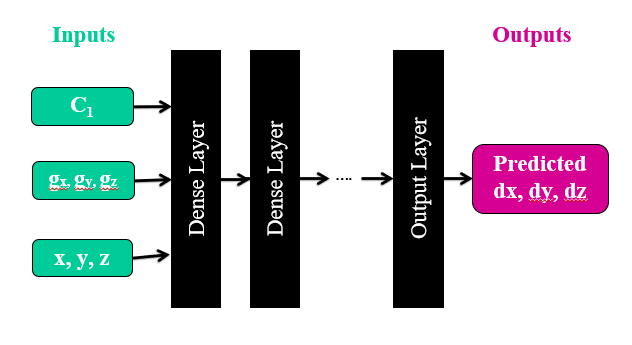
\includegraphics[scale=0.75]{Images/breast/surrogate_network.png}
    \caption{\textit{\label{fig1}The surrogate model's neural network architecture consists of three dense hidden layers and a single output layer. The inputs are fed into dense layers containing 32 neurons each. These neurons are connected to all neurons in the successive layers to increase the network's capacity. The output (prediction) is compared to the known outputs from the dataset to determine model fit.}}
\end{figure}

\subsubsection{The config file}
The configuration file (Figure \ref{fig2}) controls the inputs into the function and model as well as the parameters of the machine learning model.

\begin{figure}[H]
    \centering
    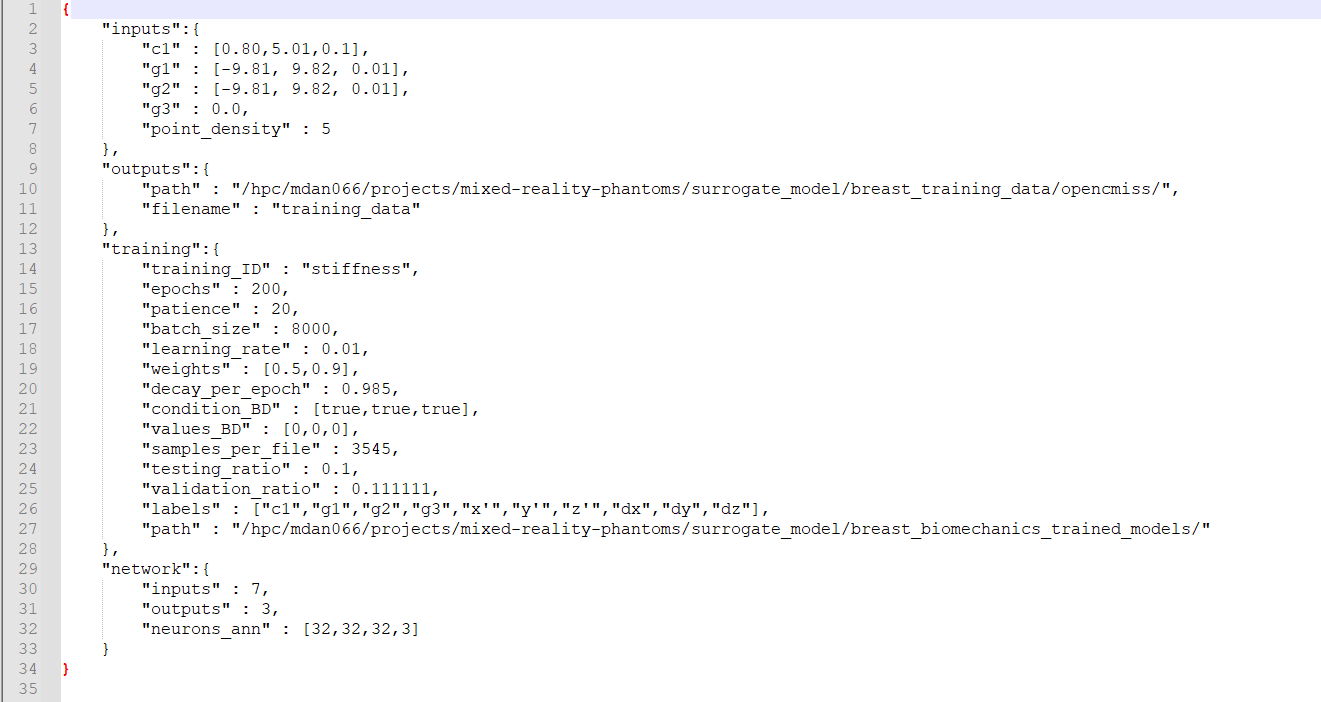
\includegraphics[scale=1.1]{Images/breast/breast_opencmiss_config.png}
    \caption{\textit{\label{fig2}Layout of the config file containing four different objects: model inputs, model outputs, training hyperparameters and network structure.}}
\end{figure}

The model's inputs and outputs are described in section 2.2.3, whilst it's parameters (training class of the file) are defined in section 2.2.4. The network's structure and definition was previously explained in section 2.2.1. 

\textbf{Note:} Pay attention to the paths under \textit{outputs} and \textit{training}. It is key to understand the provided file paths and why they are included in the file. 

% Model parameters
\subsubsection{Model parameters}
The model contains parameters that affect how the model runs and
operates (Figure \ref{fig2}). These are:

\begin{itemize}
\tightlist
\item
  \textit{epochs}: Number of times the full dataset is passed through the neural
  network.
\item
  \textit{batch\_size}: The size of each data batch. The total amount of data
  is often too large to run at once. Needs to be split into randomised batches.
\item
  \textit{learning\_rate}: Decides how far to travel in each step. A low
  learning rate is prone to long run times and gets stuck in
  local minima. A large learning rate often leads to instability.
\item
  \textit{weights}: Provides the weighting on each of the domain and dirichlet boundary.
\item
  \textit{decay\_per\_epoch}: Decides how the learning rate alters between each
  epoch with the learning rate being calculated by the current learning
  rate * the decay.
\item
  \textit{condition\_BN}: Setting if the Neumann boundary condition values are applied on the x, y, z axes.
\item
  \textit{values\_BN}: Neumann boundary condition values. 
\item
  \textit{condition\_BD}: Setting if the Dirichlet boundary condition values are applied on the x, y, z axes.
\item
  \textit{values\_BD}: Dirichlet boundary condition values. 
\item
  \textit{samples per file}: Number of samples in each file.
\item
  \textit{testing\_ratio}: The ratio of testing to training data.
\item
  \textit{validation\_ratio}: The ratio of validation to training data.
\item
  \textit{labels}: Labels the inputs and outputs.
\item
  \textit{inputs}: Number of model inputs.
\item
  \textit{outputs}: Number of model outputs.
\item
  \textit{neurons\_ann}: The neural network structure, specifically the number of neurons per layer.
\end{itemize}

%   Dataset
\subsubsection{Dataset}
The dataset should be in the format matching the labels with a full \textit{.csv} file (Figure \ref{fig3}). To add more inputs just add more columns. These csv files are stored inside the folder \textit{``breast\_training\_data``}.

\begin{figure}
\centering
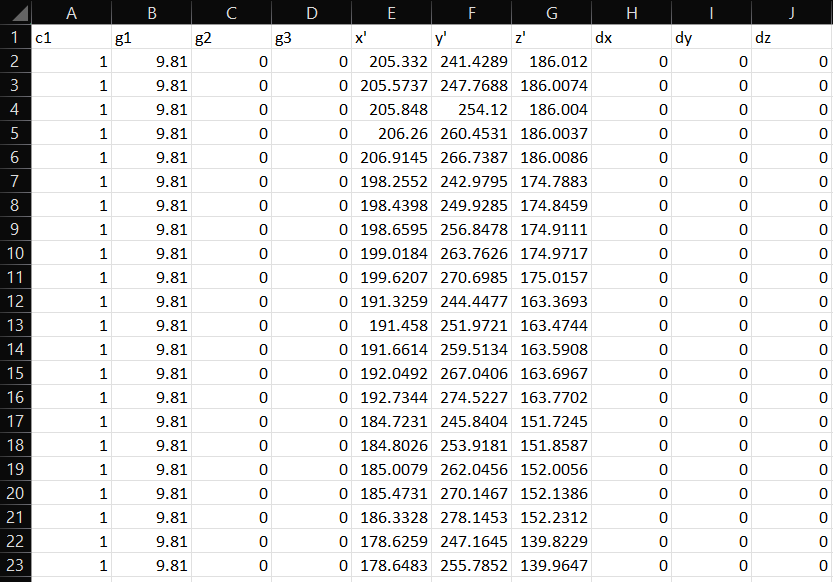
\includegraphics[scale=0.7]{Images/breast/training_data_structure.png}
\caption{\textit{\label{fig3}An example case used in the dataset for training and validating surrogate models. Note that there are seven inputs ($C_{1}$, $g_{1}$, $g_{2}$, $g_{3}$, x, y, z) and three outputs (x', y', z') per sample.}}
\end{figure}

The trained model takes a material stiffness parameter $C_{1}$, the gravity force vector $g$ = [$g_{1}$, $g_{2}$, $g_{3}$], and the reference geometry (x, y, z) to return the material point displacement (x', y', z'). The model receives a large dataset of related inputs and outputs (labels) and trains itself of the knowledge for the correct output based on each input combination. In this example, data was generated from an incompressible, homogeneous, and isotropic breast model under gravity loading using $C_{1}$ values between 0.8 kPa and 5.0 kPa in 0.1 kPa intervals (Figure \ref{fig4}).

\begin{figure}
\centering
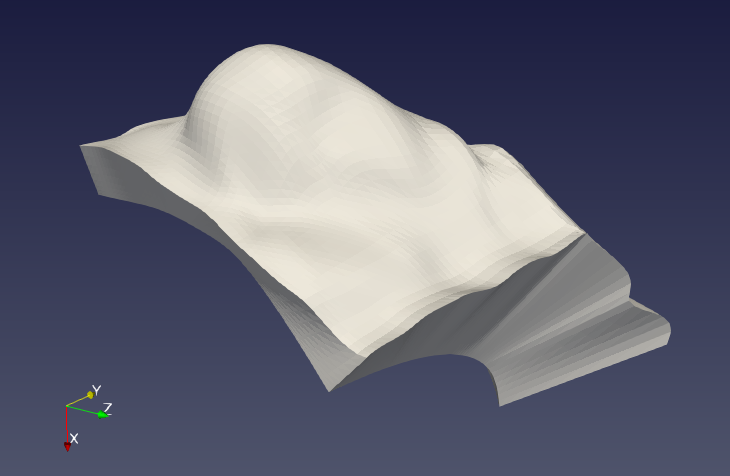
\includegraphics[scale=0.7]{Images/breast/breast_visualisation.png}
\caption{\textit{\label{fig4}The synthetic dataset was generated using a simplified breast biomechanics model of the breast. The reference configuration mesh is visualised here}} 
\end{figure}

\subsubsection{Model prediction script}


\pagebreak

%   Part II: Training surrogate models.
\section{Part II: How to train surrogate models}
This section provides the step-by-step procedure for training surrogate models. Note this is only an example and can be modified to meet your purposes. Therefore, we also discuss practical strategies for fine-tuning the model. 

\subsection{Obtaining the relevant files}
There are two approaches for obtaining the aforementioned files from the introduction to train these models: either by HPC or GitHub. 

\subsubsection{HPC Directory Structure}
This approach requires you to copy files securely from Max's HPC folder. Make sure you've copied over everything from the directory: \textit{/hpc/mdan066/projects/mixed-reality-phantoms/surrogate\_model}. We shall call this the root directory. The provided directories for the following files are relative to this directory. 

\begin{itemize}
\tightlist
\item 
\textbf{Dataset for multiple material parameters:} \textit{/breast\_training\_data/}

\item
\textbf{Configuration file:} \textit{/BioMeS/resources/data\_generation\_breast.gen}

\item
\textbf{Model script file:} \textit{/BioMeS/scripts/run\_learn\_model\_breast.py}

\end{itemize}

It is best to replicate a similar file structure in your local directory. Note back to section 2.2.2, we can change the training path (the bottom one) to a path of your choice. For example, you create a new folder \textit{trained\_models} at the same directory level as \textit{BioMeS}. 

\subsubsection{GitHub repository}
You can obtain all the required files in the provided file structure by accessing the GitHub repository: BioMeS (\url{https://github.com/seemurgh/BioMeS}). For the breast biomechanics example, please use the branch \textit{mdan066\_bbr\_mechanics}. It is best that you fork the branch onto your GitHub and clone the repository onto your local drive. Ensure that you keep the code version-controlled. For further information on source code version control, please refer to this \href{https://research-software-development-tutorials.readthedocs.io/en/latest/beginner/managing_source_code.html}{documentation}.

\subsection{Procedure for training model}

\subsubsection{Checking for GPUs to run model}\label{GPUs}
Chose a GPU which is not being used. To monitor activity in the gpus: 
\begin{itemize}
\tightlist
\item \textit{nvidia-smi -l 1} - Updates every second and gives current status. 
\item \textit{gpustat} - Shows the GPUs currently in use and key stats such as available storage space.
\end{itemize}

\subsubsection{Commands for running the model}\label{step-by-step}
The following set of commands should be ran in the terminal (for
hpc7) (Figure \ref{fig4}):

\begin{tcolorbox}[breakable, size=fbox, boxrule=1pt, pad at break*=1mm,colback=cellbackground, colframe=cellborder]
\prompt{In}{incolor}{1}{\boxspacing}
\begin{Verbatim}[commandchars=\\\{\}]
\PY{n}{module} \PY{n}{load} \PY{n}{cuda}\PY{o}{/}\PY{n}{cuda}\PY{o}{-}\PY{n}{10.1}
\end{Verbatim}
\end{tcolorbox} 
Loads the parallel computing for running on the GPUs. \\

\begin{tcolorbox}[breakable, size=fbox, boxrule=1pt, pad at break*=1mm,colback=cellbackground, colframe=cellborder]
\prompt{In}{incolor}{2}{\boxspacing}
\begin{Verbatim}[commandchars=\\\{\}]
\PY{n}{source} \PY{o}{/}\PY{n}{hpc}\PY{o}{/}\PY{n}{gmas685}\PY{o}{/}\PY{n}{programs}\PY{o}{/}\PY{n}{tensorflow\PYZus{}2\PYZus{}1\PYZus{}HPC7}\PY{o}{/}\PY{n}{bin}\PY{o}{/}\PY{n}{activate}
\end{Verbatim}
\end{tcolorbox}
Execute and start tensorflow which should change your terminal.\\

\begin{tcolorbox}[breakable, size=fbox, boxrule=1pt, pad at break*=1mm,colback=cellbackground, colframe=cellborder]
\prompt{In}{incolor}{3}{\boxspacing}
\begin{Verbatim}[commandchars=\\\{\}]
\PY{n}{cd} \PY{o}{/}\PY{n}{#your\PYZus{}folder\PYZus{}for\PYZus{}BioMeS#}\PY{o}{/}\PY{n}{BioMeS}\PY{o}{/}\PY{n}{scripts}\PY{o}{/}
\end{Verbatim}
\end{tcolorbox}
Moves to your folder containing the \textit{run\_learn\_model\_breast.py} script. \\

\begin{tcolorbox}[breakable, size=fbox, boxrule=1pt, pad at break*=1mm,colback=cellbackground, colframe=cellborder]
\prompt{In}{incolor}{4}{\boxspacing}
\begin{Verbatim}[commandchars=\\\{\}]
\PY{n}{CUDA\PYZus{}VISIBLE\PYZus{}DEVICES}\PY{o}{=}\PY{l+m+mi}{6} \PY{n}{PYTHONPATH}\PY{o}{=}\PY{o}{/}\PY{n}{hpc}\PY{o}{/}\PY{n}{mdan066}\PY{o}{/}\PY{n}{projects}\PY{o}{/}\PY{n}{mixed-reality-phantoms}\PY{o}{/}\PY{n}{surrogate_model}\PY{o}{/}\PY{n}{BioMeS}\PY{o}{/} \PY{n}{python} \PY{n}{run\PYZus{}learn\PYZus{}model\PYZus{}breast}\PY{o}{.}\PY{n}{py} \PY{n}{..}\PY{o}{/}\PY{n}{resources}\PY{o}{/}\PY{n}{data\PYZus{}generation\PYZus{}breast}\PY{o}{.}\PY{n}{gen}
\end{Verbatim}
\end{tcolorbox}
Set which GPU to use (the one you decided on earlier (example=\textit{6})), set the environment variable (PYTHONPATH=), run the model
(\textit{run\_learn\_model\_breast.py}), and put the location and name of the
configuration file (\textit{data\_generation\_breast.gen}). \\

The terminal should look like Figure \ref{fig5}, with the key model metrics from training provided in Figure \ref{fig6}.
 
\begin{figure}
\centering
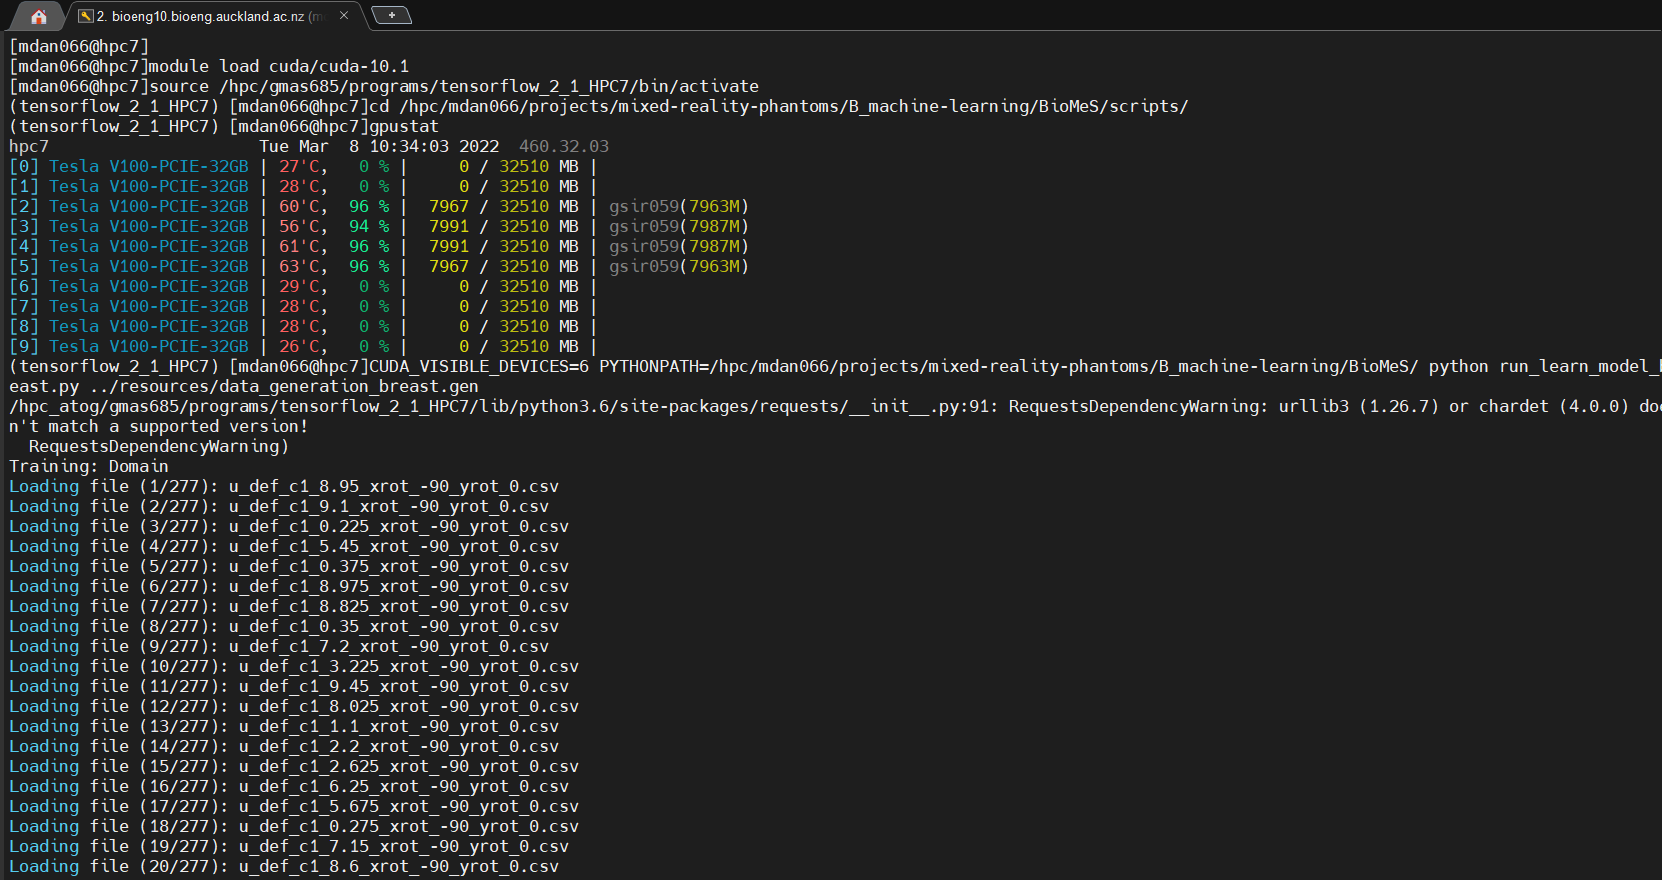
\includegraphics[scale=1.1]{Images/breast/commands/terminal_commands.png}
\caption{\textit{\label{fig5}Terminal output from the provided commands to run the model.}}
\end{figure}

\begin{figure}
\centering
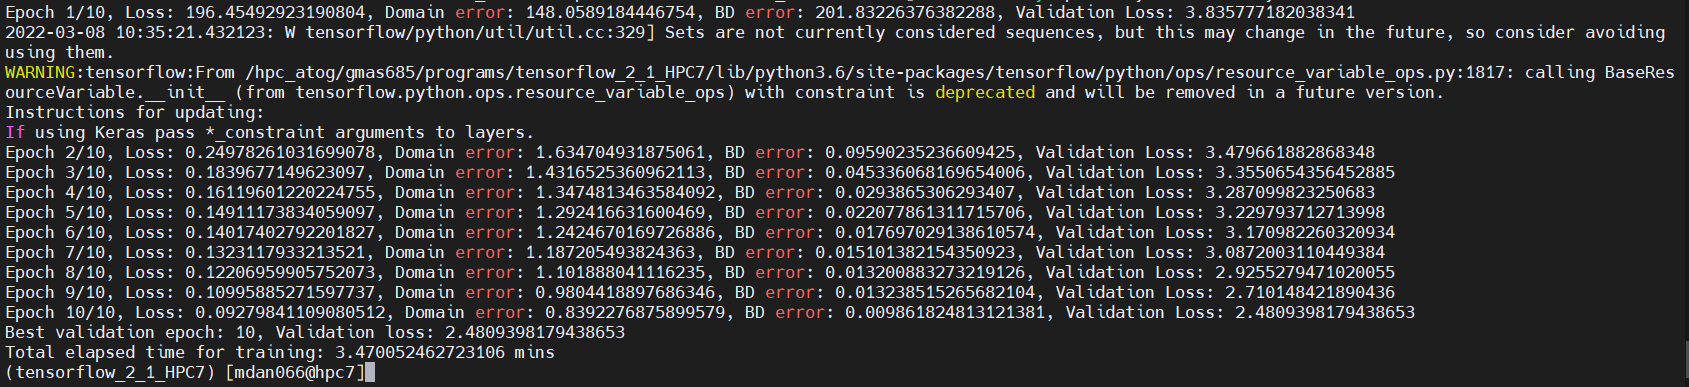
\includegraphics[scale=1.1]{Images/breast/commands/epochs.PNG}
\caption{\textit{\label{fig6}Key metric outputs from training the model. Validation loss indicates the true model performance and the best model uses the network parameters from the best validation epoch.}}
\end{figure}

Note that Figures 5 and 6 were generated for a different model and therefore not representative for data generated from the OpenCMISS model.

\subsubsection{Visualising model on Tensorboard}
Once training is completed, we can visualise the validation loss using TensorBoard on a browser. This tracks and plots the metrics (loss and accuracy) involved in a machine learning workflow. One of TensorBoard's main benefits is that we don't need additional code within the scripts to save and write information. Instead, data can be saved in graph execution and not taken out of the GPU. This enables cross-platform applications, flexibility in use and larger model trainings. 

Tensorboard was initialised in the \textit{run\_learn\_model.py} script to plot the training metrics of the surrogate model. 
\begin{tcolorbox}[breakable, size=fbox, boxrule=1pt, pad at break*=1mm,colback=cellbackground, colframe=cellborder]
\prompt{In}{incolor}{5}{\boxspacing}
\begin{Verbatim}[commandchars=\\\{\}]
\PY{n}{tensorboard}\PY{o}{_}\PY{n}{log} \PY{o}{=} \PY{n}{tf}\PY{o}{.}\PY{n}{keras}\PY{o}{.}\PY{n}{callbacks}\PY{o}{.}\PY{n}{TensorBoard}\PY{o}{(}\PY{n}{log}\PY{o}{_}\PY{n}{dir} \PY{o}{=} \PY{n}{output}\PY{o}{_}\PY{n}{path}\PY{o}{)}
\PY{n}{tensorboard}\PY{o}{_}\PY{n}{log}\PY{o}{.}\PY{n}{set}\PY{o}{_}\PY{n}{model}\PY{o}{(}\PY{n}{surrogate}\PY{o}{_}\PY{n}{model}\PY{o}{)}
\end{Verbatim}
\end{tcolorbox} 

The key metrics from Figure \ref{fig6} are stored as \textit{logs} which is displayed on the TensorBoard interface. 
\begin{tcolorbox}[breakable, size=fbox, boxrule=1pt, pad at break*=1mm,colback=cellbackground, colframe=cellborder]
\prompt{In}{incolor}{6}{\boxspacing}
\begin{Verbatim}[commandchars=\\\{\}]
\PY{n}{logs} \PY{o}{=} \PY{o}{\{}logs = {'Loss': train_loss.result(), 'Domain Error': domain_error.result(), 'Dirichlet BD Error': BD_error.result(), 'Validation Loss': validation_loss.result()}\PY{o}{\}}
tensorboard_log.on_epoch_end(epoch, logs)
\end{Verbatim}
\end{tcolorbox}

Tensorboard is typically executed on your local machine's command line rather than HPC as HPC's HTTP ports are closed for security reasons. The command to run Tensorboard and visualise your model's key metrics are: 
\begin{tcolorbox}[breakable, size=fbox, boxrule=1pt, pad at break*=1mm,colback=cellbackground, colframe=cellborder]
\prompt{In}{incolor}{7}{\boxspacing}
\begin{Verbatim}[commandchars=\\\{\}]
tensorboard --logdir "directory of tf-event files"
\end{Verbatim}
\end{tcolorbox} 
where the directory of tf-event files are  \textit{/breast\_biomechanics\_trained\_models/case\_folder/train} from the root directory. There should be only one event file per \textit{case\_folder}, with the following name convention: \textit{events.out.tfevents.<TIMESTAMP>.<MACHINE\_NAME>}. The outputs are visualised in Figure \ref{fig7}: 

\begin{figure}
\centering
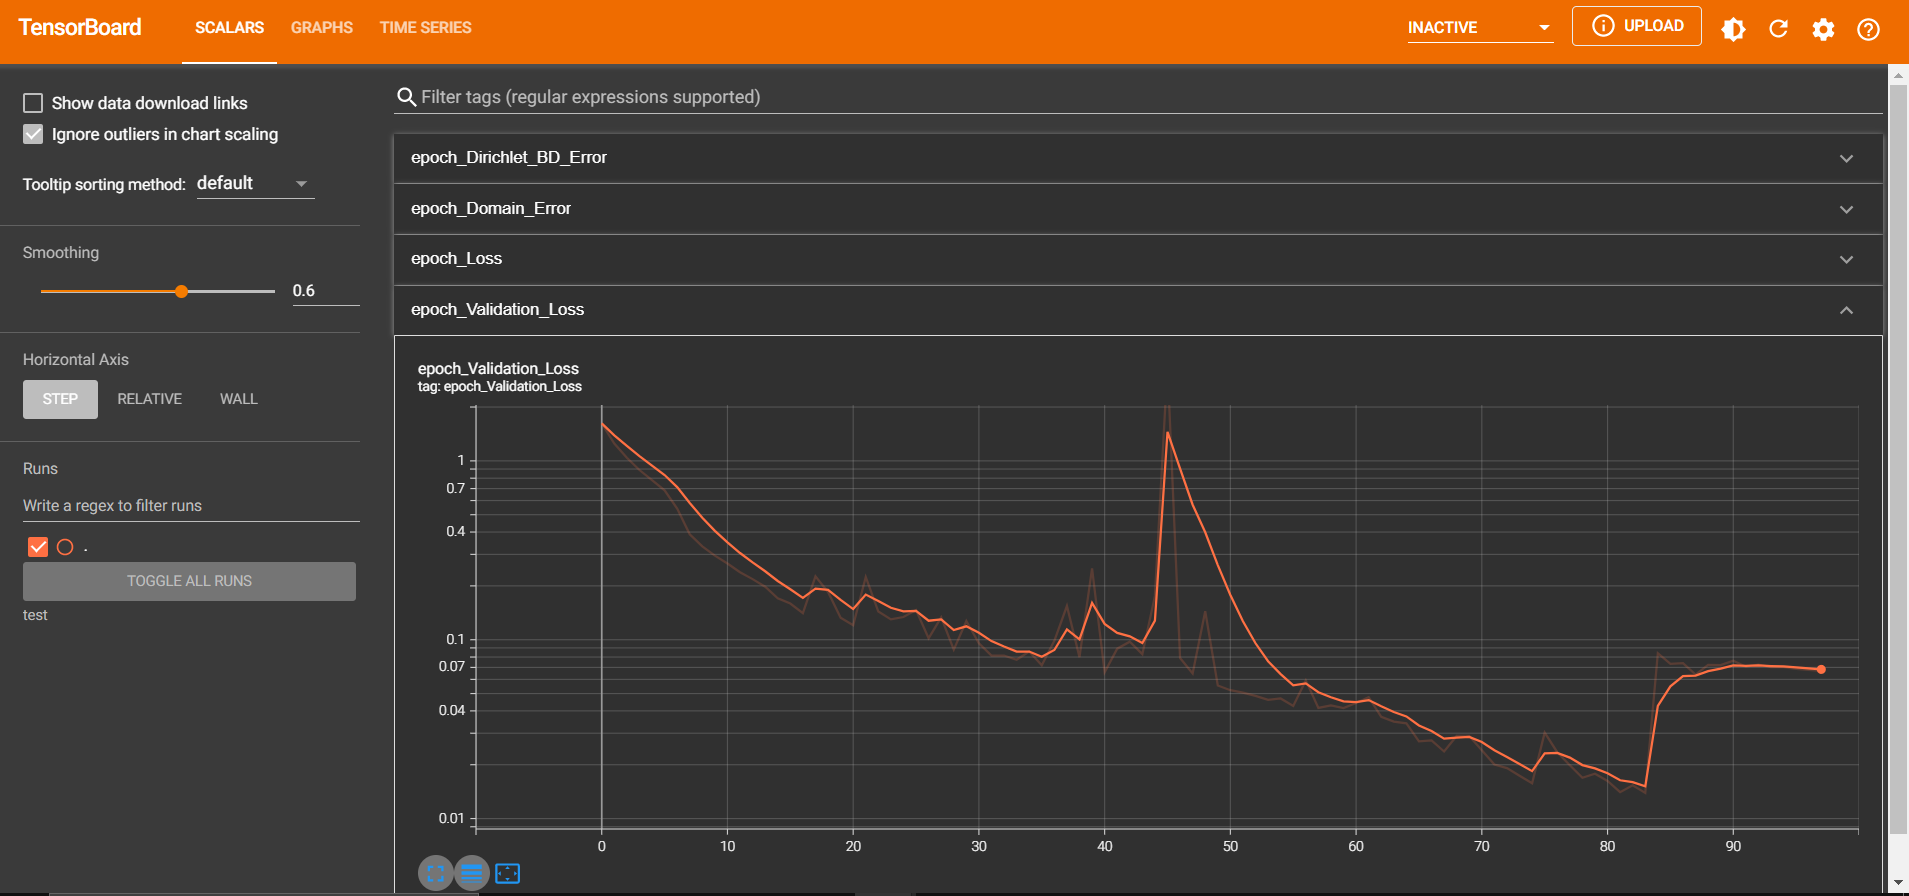
\includegraphics[scale=1.1]{Images/breast/tensorboard.png}
\caption{\textit{\label{fig7}Key metric outputs (Domain error, BD error, Validation loss) visualised on Tensorboard. Note that the validation loss is on the y-axis (in log-scale) and number of epochs is on the x-axis.}}
\end{figure}

\subsection{Use trained surrogate model to predict material point displacements}
We can check how well the surrogate model predicts the material point displacements of the breast using the script \textit{plot\_model\_error.py}. This loads in the most recently trained surrogate model (see path at \textit{cfg["training"]["path"]+"saved\_model"}) and takes in the following arguments.
\begin{itemize}
    \item sys.argv[2]: the case file of interest from the synthetic dataset (in this case, \textit{``training\_data\_c1\_3.0\_g1\_-9.81\_g2\_0.0\_g3\_0.0.csv``}).
    \item cfg["outputs"]["path"] is the directory where synthetic dataset files are located. 
    \item "g1" (x-component of gravity force) is the parameter you want to estimate. 
    \item 9.81 is the parameter value you input into the model (in this case, this represents the x-component of the gravity force in the supine orientation).
\end{itemize}
\newline

To perform the prediction and visualise its accuracy, run the following command:
\begin{tcolorbox}[breakable, size=fbox, boxrule=1pt, pad at break*=1mm,colback=cellbackground, colframe=cellborder]
\prompt{In}{incolor}{4}{\boxspacing}
\begin{Verbatim}[commandchars=\\\{\}]
\PY{n}{CUDA\PYZus{}VISIBLE\PYZus{}DEVICES}\PY{o}{=}\PY{l+m+mi}{6} \PY{n}{PYTHONPATH}\PY{o}{=}\PY{o}{/}\PY{n}{hpc}\PY{o}{/}\PY{n}{mdan066}\PY{o}{/}\PY{n}{projects}\PY{o}{/}\PY{n}{mixed-reality-phantoms}\PY{o}{/}\PY{n}{surrogate_model}\PY{o}{/}\PY{n}{BioMeS}\PY{o}{/} \PY{n}{python} \PY{n}{plot\PYZus{}model\PYZus{}error}\PY{o}{.}\PY{n}{py} \PY{n}{..}\PY{o}{/}\PY{n}{resources}\PY{o}{/}\PY{n}{data\PYZus{}generation\PYZus{}breast}\PY{o}{.}\PY{n}{gen} \PY{n}{training\PYZus{}data\PYZus{}c1\PYZus{}3.0\PYZus{}g1\PYZus{}-9.81\PYZus{}g2\PYZus{}0.0\PYZus{}g3\PYZus{}0.0}\PY{o}{.}\PY{n}{csv} 
\end{Verbatim}
\end{tcolorbox}


This script outputs five main metrics, as computed below in equations 2-6 below. 
\textbf{Mean absolute global error: }
\begin{itemize}
    \begin{equation}
         \overline{\epsilon} = \frac{\sum_{i=1}^{N} \sqrt{(ux_{i} - \hat{u}x_{i})^2 + (uy_{i} - \hat{u}y_{i})^2 + (uz_{i} -\hat{u}z_{i})^2}}{N}
    \end{equation}
\end{itemize}

\textbf{Standard deviation: }
\begin{itemize}
    \begin{equation}
         \sigma_{\epsilon} = \frac{\sum_{i=1}^{N}\sqrt{(ux_{i} - \hat{u}x_{i} - \overline{\epsilon})^2 + (uy_{i} - \hat{u}y_{i} - \overline{\epsilon})^2 + ((uz_{i} -\hat{u}z_{i} - \overline{\epsilon})^2}}{N}
    \end{equation}
\end{itemize}

\textbf{Mean displacement: }
\begin{itemize}
    \begin{equation}
        \overline{u} = \frac{\sqrt{ux_{i}^2 + uy_{i}^2 + uz_{i}^2}}{N}
    \end{equation}
\end{itemize}

\textbf{Min displacement: }
\begin{itemize}
    \begin{equation}
        u_{min} = min(\sqrt{ux_{i}^2 + uy_{i}^2 + uz_{i}^2})    
    \end{equation}
\end{itemize}

\textbf{Max displacement: }
\begin{itemize}
    \begin{equation}
        u_{max} = max(\sqrt{ux_{i}^2 + uy_{i}^2 + uz_{i}^2})    
    \end{equation}
\end{itemize}

For this example, we get the following output. \\
\\
\textbf{Mean absolute global error}: $0.247 \pm 0.244$ mm. \\
\textbf{Mean displacement}: \SI{0.970}{mm}. \\
\textbf{Displacement range}: $[0.001, 12.597]$ mm. 

\subsection{Visualise surrogate model predictions and errors}
From the same script \textit{plot\_model\_error.py}, we can visualise the predicted displacement field and the errors associated with this prediction. The prediction for a 3.0 kPa breast model in the prone (Figure 8) and supine (Figure 9) orientations are shown below. 

\begin{figure}
\centering
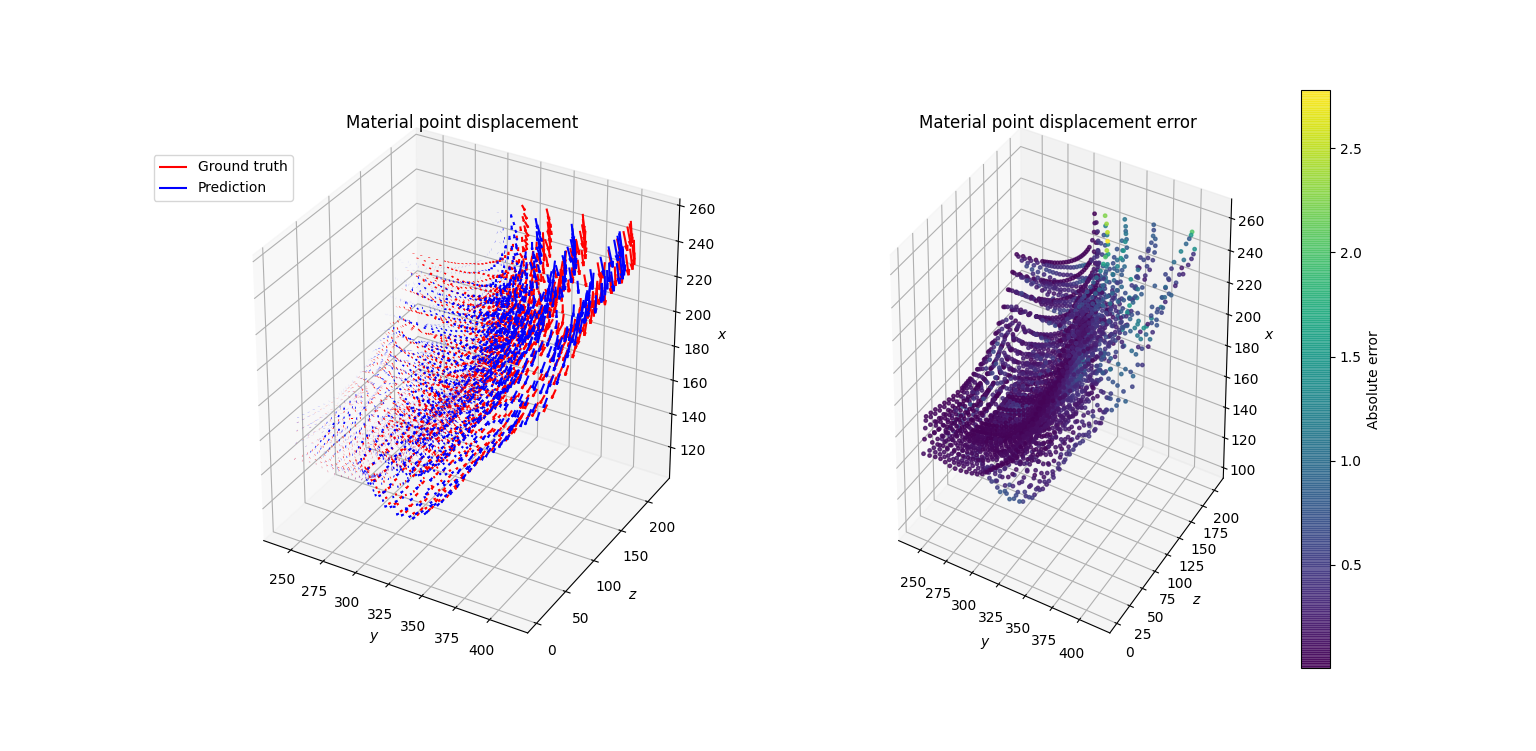
\includegraphics[scale=1.0]{Images/breast/3.0_prone_model.png}
\caption{\textit{\label{fig8}Model prediction for gravity force in prone orientation (C_1 = \SI{3.0}{kPa}).}}
\end{figure}

\begin{figure}
\centering
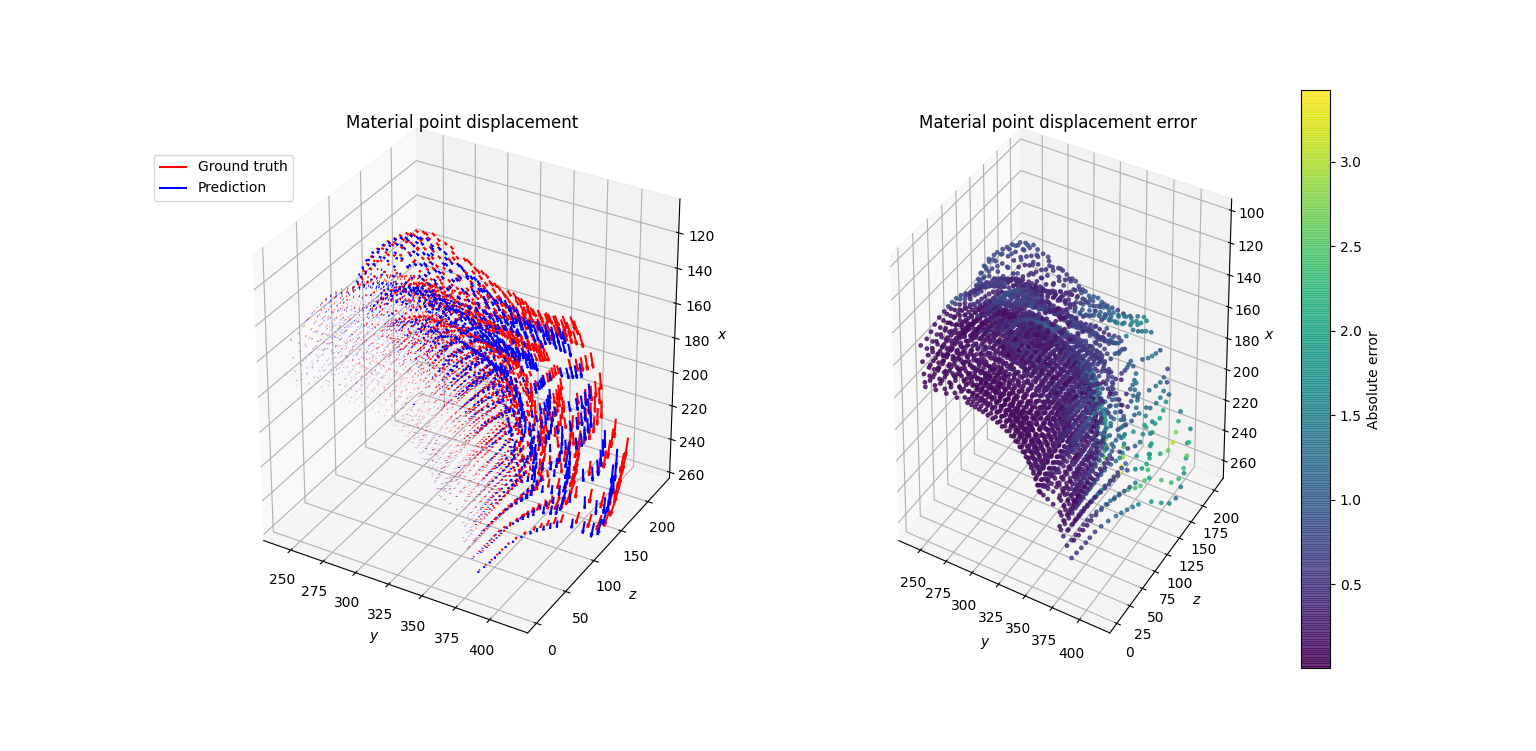
\includegraphics[scale=1.0]{Images/breast/3.0_supine_model.png}
\caption{\textit{\label{fig9}Model prediction for gravity force in supine orientation (C_1 = \SI{3.0}{kPa}).}}
\end{figure}

\pagebreak

%   Part III
\section{Part III: Parameter estimation}

\pagebreak

\section{Part IV: Practical strategies/sanity checks for model training}
When running these models, these are some practical considerations and checks to help debug the code, or improve the training process.

If you suspect that your loss function outputs seem off: 
\begin{itemize}
    \item Check that the input \& output variables fed to the network are the same as the config file. 
    \item Stop the training dataset from shuffling to make the check easier. 
    \item Compute the loss function output for an arbitrary sub-section of the data per epoch (i.e. mini batch). Compare this to your computation done by-hand. \\
\end{itemize}

\textbf{Mention something about non-convex problems.} \\

Sometimes the validation loss does not improve significantly over many epochs. This suggests that the surrogate model is not learning effectively. Some tweaks to consider are: 

\begin{itemize}
    \item Make the weight for domain error = 0. This ensures we're only training the Dirichlet BCs. 
    \item Change the learning rate. Higher learning rates lead to large weight updates which results in oscillations around the minima. However, this is recommended for stochastic or mini-batch gradient descent where only subsets of the dataset are sampled and large learning rates would improve the exploration of the function space. Too small a learning rate leads to slow convergence towards a global minima or being stuck in an undesirable local minima without the opportunity for exploration. Ensure the learning rates differ in orders of magnitude (i.e. 0.1, 0.01, 0.001).
    \item Vary your batch size. Smaller batch sizes can lead to imprecise approximations of the objective function's gradient in each batch. In comparsion to larger batch sizes, there are more gradient evaluations which enables greater exploration of the function space, and therefore improve the model's ability to generalise.
    \item Increase the number of maximum epochs to a very high number. More epochs typically enables better training. An early stopping condition can be implemented to stop training once the model performance does not improve any further over a certain number of epochs (therefore saving unnecessary computational costs). 
    \item A large number of epochs may lead to overfitting of the model. However, we want to see when network overfits and stop training when this happens. The extracted results will be independent to the number of epochs, as we are only interested in the epoch with the lowest validation loss score. 
    \item Add more neurons to each layer or increase the number of layers in the network. More layers typically increases training time significantly.  
    \item Perform sensitivity analysis of optimisation parameters (learning rate, batch size), and architecture parameters (number of hidden layers and neurons per layer). Use a grid search for this systematic evaluation.
    \item Use the test loss as the metric for sensitivity analysis. Validation loss can be biased, as it estimates the generalised performance of the model in a way that is biased to fitting to the data. Test loss is an unbiased evaluation of the final model fit. (\textbf{Not too sure about this, check again.})\\   
\end{itemize}

In general, best to conduct training on HPC as it satisfies the substantial GPU storage requirements. However, it is best to debug and prototype locally. This provides more freedom for you to try things out or install particular softwares without affecting other HPC users (HPC has certain restrictions on installation for this reason). 

\pagebreak

%   Contributors
\section{Contributors}
\href{https://unidirectory.auckland.ac.nz/profile/scre583}{Stephen Creamer} created the original iteration of this documentation and the basis for Part I. 

\href{https://unidirectory.auckland.ac.nz/profile/psam012}{Dr Prasad Babarenda Gamage} contributed to developing the surrogate models and provided practical insights into programming and documentation best practices.   

\href{https://unidirectory.auckland.ac.nz/profile/g-masotalou}{Dr Gonzalo Maso Talou} is the main developer of the surrogate model \& parameter estimation framework, and provided practical insights into machine learning in Part II.

%   Bibliography
\section{References}
    
\end{document}